\chapter{Automatizované testování}
\label{chap:testing}

Pro zajištění kvality a stability systému Evolio existuje v rámci firemní infrastruktury sada automatizovaných UI testů. Tyto testy simulují reálné chování uživatele v prohlížeči a slouží jako regresní testování po nasazení nové verze aplikace. V rámci praxe jsem se do tohoto projektu zapojil -- rozšiřoval jsem stávající sadu o nové testovací scénáře a průběžně pečoval o funkčnost již existujících testů.

\section{Metodika a zařazení v testovací pyramidě}

Automatizované testování softwaru bývá zpravidla strukturováno podle tzv. \textit{testovací pyramidy} \cite{fowler_test_pyramid, meszaros_xunit}, která rozlišuje tři vrstvy testů podle granularity a rychlosti zpětné vazby:

\begin{table}[H]
\centering
\caption{Vrstvy testovací pyramidy a jejich pokrytí v projektu Evolio}
\label{tab:test_pyramid}
\begin{tabular}{|l|p{4cm}|p{3.5cm}|p{3.5cm}|}
\hline
\textbf{Vrstva} & \textbf{Účel} & \textbf{Nástroje v Evoliu} & \textbf{Moje zapojení} \\ \hline
Unit testy & Izolované testování jednotek kódu (metody, třídy). & NUnit, Moq (v dílčích modulech). & Minimální -- moduly, na kterých jsem pracoval, mají nízké pokrytí unit testy. \\ \hline
Integrační testy & Ověření spolupráce více komponent (služba + DB). & Vlastní framework nad .NET + testovací SQL instance. & Žádné -- nebyly předmětem praxe. \\ \hline
UI / E2E testy & Simulace uživatele v prohlížeči; validace end-to-end scénářů. & Selenium WebDriver, NUnit, Boa.Constrictor. & Hlavní oblast praxe -- rozšiřování a údržba. \\ \hline
\end{tabular}
\end{table}

UI testy stojí na vrcholu pyramidy; jsou nejpomalejší a nejnáchylnější k nestabilitě (tzv. \textit{flaky tests}), ale zároveň poskytují nejbližší aproximaci reálného uživatelského scénáře. Jejich hodnota spočívá v tom, že odhalí chyby vznikající na rozhraní mezi vrstvami -- například selhání komunikace mezi frontendem a backendem nebo chybně vyrenderované UI prvky, které unit test nemůže odhalit.

\section{Strategie a nástroje}

Jako technologický základ byl zvolen framework \textbf{Selenium WebDriver} \cite{selenium_docs}, který je v .NET prostředí de facto standardem pro automatizaci webových prohlížečů. Pro samotné spouštění testů a validaci podmínek (assertions) je využit framework \textbf{NUnit} \cite{nunit_docs} (atributy \texttt{[Test]}, \texttt{[SetUp]}, \texttt{[TearDown]}).

\subsection{Volba návrhového vzoru: Screenplay místo Page Object Modelu}

Pro organizaci testovacího kódu existují dva převládající návrhové vzory. Jejich srovnání shrnuje tabulka \ref{tab:pom_vs_screenplay}.

\begin{table}[H]
\centering
\caption{Porovnání Page Object Model a Screenplay Pattern}
\label{tab:pom_vs_screenplay}
\begin{tabular}{|l|p{5cm}|p{5cm}|}
\hline
\textbf{Aspekt} & \textbf{Page Object Model (POM)} & \textbf{Screenplay Pattern} \\ \hline
Hlavní abstrakce & Stránka (třída reprezentující jednu obrazovku). & Herec (Actor) a jeho akce. \\ \hline
Organizace kódu & Metody jsou vázány na stránku. & Akce jsou samostatné, znovupoužitelné. \\ \hline
Čitelnost testu & Procedurální styl. & Deklarativní, čitelný jako přirozený jazyk. \\ \hline
Škálovatelnost & Při růstu se objevují „God Object" třídy. & Lepší kompozice; nové akce bez zásahu do stránek. \\ \hline
Křivka učení & Nízká. & Vyšší -- vyžaduje pochopení SOLID principů. \\ \hline
\end{tabular}
\end{table}

Projekt UI testů v Evoliu využívá \textbf{Screenplay Pattern} \cite{knight_screenplay} implementovaný pomocí knihovny \textbf{Boa.Constrictor} \cite{boa_constrictor}. Tento přístup se zaměřuje na to, \emph{co} uživatel (Actor) dělá, spíše než na strukturu stránek, a odpovídá principům SOLID -- zejména Single Responsibility Principle, neboť každá akce má jediný důvod ke změně \cite{martin_clean_architecture}.

Základní stavební kameny architektury jsou:
\begin{itemize}
    \item \textbf{Actor (Tester):} Entita provádějící test. V našem případě je instanciována v \texttt{BaseTest} třídě.
    \item \textbf{Task:} Složitější úloha skládající se z více kroků (např. \texttt{Login.WithSessionCredentials()}).
    \item \textbf{Interaction:} Atomická akce (např. \texttt{Click.On(...)}, \texttt{SendKeys.To(...)}).
    \item \textbf{Question:} Dotaz na stav aplikace (např. \texttt{Appearance.Of(...)}, \texttt{ValueAttribute.Of(...)}).
\end{itemize}

\section{Implementace testovacích scénářů}

Testy jsou organizovány do logických celků podle agend (Podatelna, Případy, Subjekty). Následující ukázka demonstruje strukturu CRUD testu pro vytvoření nového subjektu.

\subsection{Příklad: Vytvoření subjektu}
Testovací metoda dodržuje princip \textbf{Arrange-Act-Assert} \cite{beck_tdd}. Využívá fluent syntaxi, která činí test čitelným téměř jako přirozený jazyk.

\begin{lstlisting}[language={[Sharp]C}, caption={Ukázka testu vytvoření subjektu pomocí Screenplay patternu}]
[Test]
public void CreateSubject_Manually_ShouldSucceed()
{
    // Arrange: Priprava dat
    string name = "Testovaci Subjekt " + Guid.NewGuid();
    string ico = "12345678";

    // Act: Provedeni akci (Navigace -> Vyplneni formulare -> Ulozeni)
    Tester.AttemptsTo(Navigate.ToUrl(SubjectPage.Url));
    Tester.AttemptsTo(Click.On(SubjectPage.AddButton));

    Tester.AttemptsTo(SendKeys.To(SubjectForm.NameInput, name));
    Tester.AttemptsTo(SendKeys.To(SubjectForm.IcoInput, ico));

    Tester.AttemptsTo(Click.On(SubjectForm.SaveButton));

    // Assert: Overeni vysledku
    // Cekame, az se objevi notifikace o uspechu
    Tester.WaitsUntil(Appearance.Of(SubjectPage.SuccessToast), IsEqualTo.True());

    // Overeni, ze se subjekt nacetl v detailu
    Tester.AskingFor(Text.Of(SubjectPage.DetailHeader)).Should().Contain(name);
}
\end{lstlisting}

\subsection{Správa testovacích dat a izolace}

Zajištění opakovatelnosti testů je v UI prostředí kritické, neboť chyby v datové izolaci vedou k nejčastější příčině nestabilních testů. V projektu jsou uplatňovány tyto principy:
\begin{itemize}
    \item \textbf{Unikátní identifikátory} -- každý vytvářený záznam dostává na vstupu \texttt{Guid.NewGuid()} v názvu, takže nedojde ke kolizi s artefakty z předchozích běhů.
    \item \textbf{Izolovaná databáze} -- testy se spouštějí proti samostatné testovací instanci SQL Serveru, která je resetována před každým release buildem.
    \item \textbf{Session credentials} -- přihlášení je sdíleno napříč testy v rámci jedné třídy přes atribut \texttt{[OneTimeSetUp]}, což zkracuje celkový běh.
\end{itemize}

\subsection{Ošetření nestability (flakiness)}

Explicitní čekání pomocí \texttt{Tester.WaitsUntil(...)} eliminuje významnou část nestability způsobenou asynchronním načítáním dat. Tam, kde je chování časově nedeterministické (např. závislost na AI API nebo na externí službě), je použit interní retry mechanismus knihovny Boa.Constrictor, který akci opakuje s definovaným intervalem a maximálním počtem pokusů.

\section{Integrace do CI/CD (Azure DevOps)}

Testovací projekt je integrován do procesu kontinuální integrace a nasazování (CI/CD) na platformě \textbf{Azure DevOps} \cite{azure_devops_docs}, kde jsem se podílel na správě buildovacích a release pipeline.

\subsection{Spouštění testů}
Testy jsou automaticky spouštěny po každém nasazení nové verze do testovacího prostředí. Běží na vzdáleném virtuálním stroji v prohlížeči Google Chrome v režimu headless, což zkracuje dobu běhu a umožňuje paralelní spouštění více testovacích běhů.

\begin{figure}[h]
    \centering
    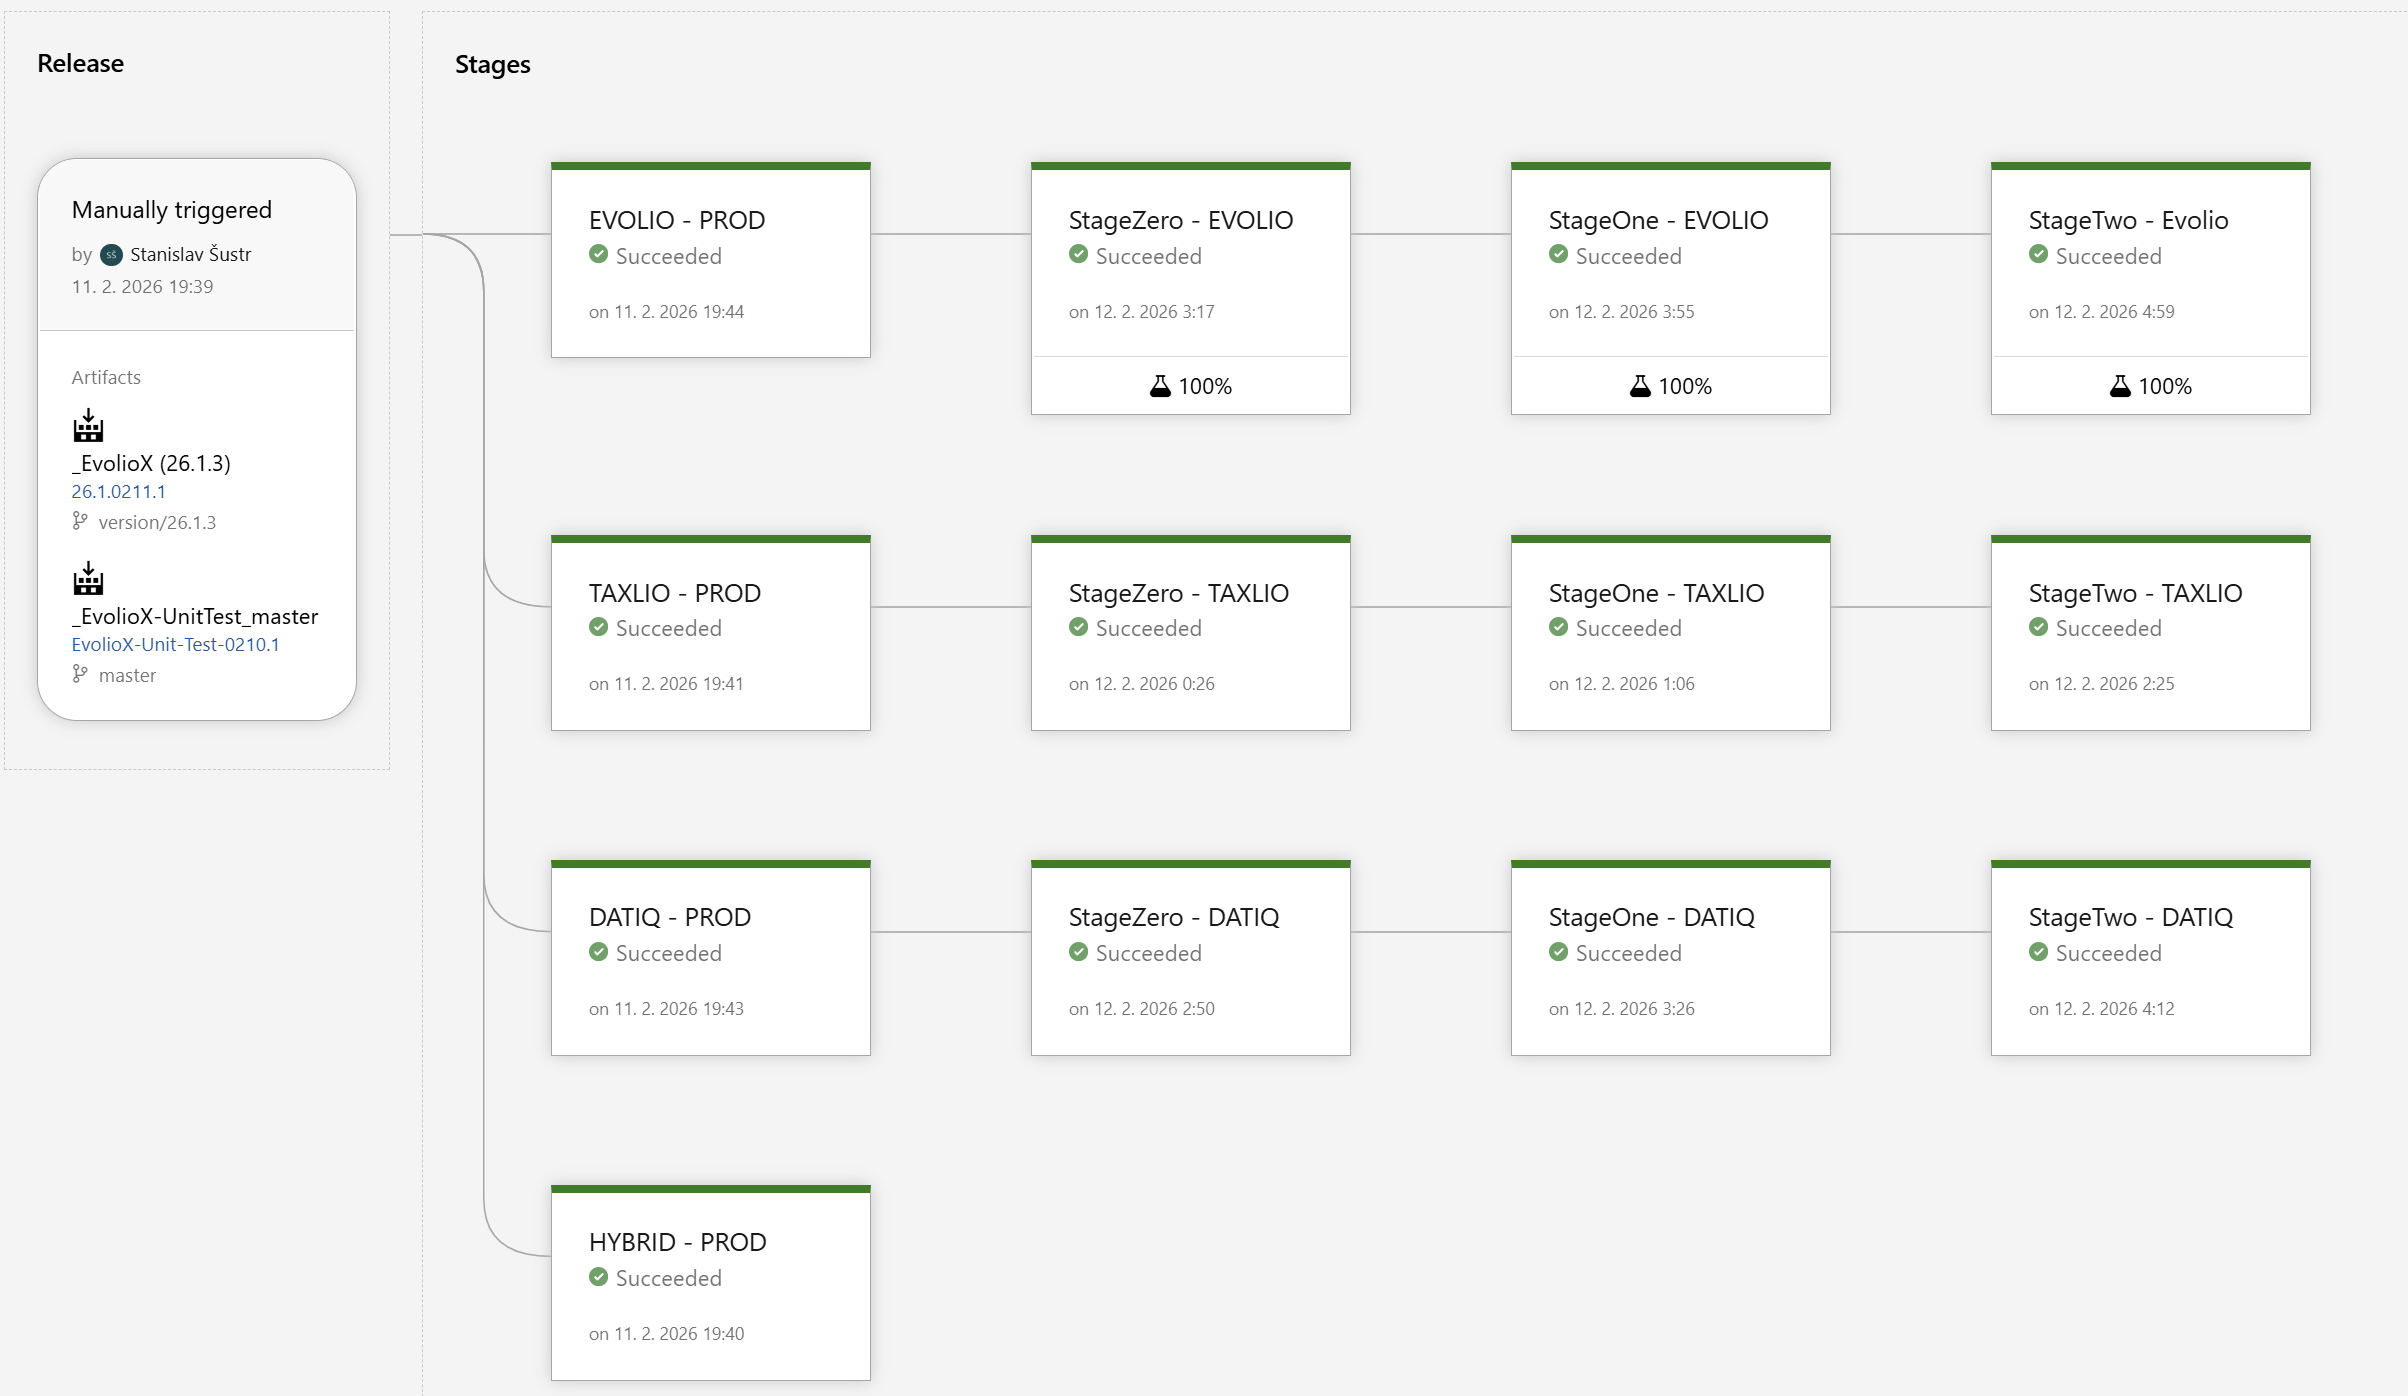
\includegraphics[width=1\textwidth]{Figures/DevOpsPipeline.png}
    \caption{Ukázka úspěšného běhu automatizovaných testů v release pipeline Azure DevOps}
    \label{fig:azure_devops}
\end{figure}

\subsection{Diagnostika chyb}
Pro efektivní řešení problémů je implementován mechanismus, který v případě pádu testu:
\begin{enumerate}
    \item Automaticky pořídí \textbf{screenshot} obrazovky v momentě chyby.
    \item Uloží systémové logy a stack trace.
    \item Tyto artefakty připojí k výsledku testu v Azure DevOps Dashboardu.
\end{enumerate}

Tato automatizace výrazně zrychluje proces debugování, protože umožňuje okamžitě identifikovat, zda chyba nastala v aplikaci (např. validační hláška) nebo v testu samotném.

\section{Přínos testovací sady}

Sada automatizovaných testů již v průběhu mé praxe opakovaně odhalila regresní chyby ještě před nasazením k zákazníkům -- konkrétní příklad je uveden v kapitole \ref{chap:evaluation}. Současný stav pokrývá klíčové CRUD operace hlavních agend (Podatelna, Případy, Subjekty, Fakturace) a jeho rozšíření o nové scénáře bylo jednou z mých průběžných činností. Pro další růst kvality by bylo vhodné doplnit nižší vrstvy pyramidy -- zejména integrační testy serverové logiky Add-inů, kde jsou dnes regrese odhalovány až UI testy, což je nákladnější z hlediska doby běhu a diagnostiky.
